\documentclass{beamer}

\mode<presentation>
{
  \usetheme{AnnArbor}
  \usecolortheme{beaver}
  %\usefonttheme{serif}
}


\usepackage[utf8]{inputenc}
\usepackage{default}
\usepackage[caption=false]{subfig}
\usepackage{graphicx}
%\usepackage{pslatex}
\usepackage{setspace}
\usepackage{hyperref}
\usepackage{amssymb}
\usepackage{epstopdf}
\usepackage{listings}
\usepackage{color}
\usepackage{amsmath}
\usepackage{tikz}
\usepackage{mathtools}
\usepackage[caption=false]{subfig}

%Equations/Entries
\newcommand{\beq}{\begin{equation}}
\newcommand{\bequo}{\begin{quotation}}
\newcommand{\beqa}{\begin{eqnarray}}
\newcommand{\eeq}{\end{equation}}
\newcommand{\leeq}[1]{\label{#1}\end{equation}}
\newcommand{\equo}{\end{quotation}}
\newcommand{\eeqa}{\end{eqnarray}}
\newcommand{\non}{\nonumber}
\newcommand{\mx}{\mbox}
\newcommand{\mxf}[1]{\mbox{\footnotesize{#1}}}
\newcommand{\lb}{\label}
\newcommand{\fr}[1]{(\ref{#1})}
\newtheorem{entry}{}[section]
\newcommand{\bent}[1]{\vspace*{-2cm}\hspace*{-1cm}\begin{entry}\lb{e{#1}}\rm}
\newcommand{\eent}{\end{entry}}
\newcommand{\fre}[1]{{\bf\ref{e{#1}}}}
\newcommand{\Emark}{$\sqcap\hspace{-2.7mm}\sqcup$}
\newcommand{\sEmark}{{\fns $\sqcap\hspace{-2.3mm}\sqcup$}}
\newcommand{\fn}{\footnote}


%Greek Letters
\renewcommand{\a}{\alpha}
\renewcommand{\b}{\beta}
\newcommand{\g}{\gamma}
\newcommand{\G}{\Gamma}
\renewcommand{\d}{\delta}
\renewcommand{\th}{\theta}
\renewcommand{\k}{\kappa}
\newcommand{\Th}{\Theta}
\newcommand{\D}{\Delta}
\newcommand{\e}{\epsilon}
\newcommand{\ep}{\varepsilon}
\newcommand{\s}{\sigma}
\renewcommand{\S}{\Sigma}
\newcommand{\w}{\omega}
\newcommand{\W}{\Omega}
\newcommand{\al}{\alpha}
\newcommand{\bet}{\beta}
\newcommand{\gam}{\gamma}
\newcommand{\lam}{\lambda}
\newcommand{\Lam}{\Lambda}
\newcommand{\eps}{\varepsilon}
\newcommand{\ichi}\sichi
\renewcommand{\ni}{\sni}
\renewcommand{\r}{\rho}
\renewcommand{\t}{\tau}
\newcommand{\ph}{\varphi}
\newcommand{\sichi}{{\mbox{{\footnotesize I}}}}
\newcommand{\sni}{{\mbox{{\footnotesize II}}}}

%color2010/6/9
\newcommand{\red}{\color{red}}
\newcommand{\blue}{\color{blue}}
\newcommand{\green}{\color{green}}
\definecolor{gray}{rgb}{0.5, 0.5, 0.5}
\newcommand{\gray}{\color{gray}}

%Derivatives
\newcommand{\pder}[2]{\frac{\partial {#1}}{\partial {#2}}}
\newcommand{\pdert}[2]{\frac{\partial^2 {#1}}{\partial {#2}^2}}
\newcommand{\fder}[2]{\frac{\delta {#1}}{\delta {#2}}}
\newcommand{\PDD}[3]{\left.\frac{\partial^{2}{#1}}{\partial{#2}^{2}}\right|_{#3}
}
\newcommand{\PD}[3]{\left.\frac{\partial{#1}}{\partial{#2}}\right|_{#3}}
\newcommand{\der}[2]{\frac{d {#1}}{d {#2}}}

\renewcommand{\deg}{^\circ}
\newcommand{\com}{{\bf [C] }}
\newcommand{\cend}{\Emark\[\]\vspace*{-1. cm}}
\newcommand{\x}{\times}

%My commands
\newcommand{\win}{\ddot\smile}
\newcommand{\lose}{\ddot\frown}
\newcommand{\avg}[1]{\left \langle #1 \right \rangle}
\newcommand{\E}[1]{\ensuremath{\times10^{#1}}}
\newcommand{\abs}[1]{\ensuremath{\left | #1 \right |}}
\newcommand{\paren}[1]{\left(#1\right)}
\newcommand{\recip}[1]{\frac{1}{#1}}
\newcommand{\ex}[1]{\mathbb{E}[#1]}
\newcommand{\bprob}[1]{\textbf{#1~---}}
\newcommand{\unitv}[1]{\ensuremath{\mathbf{\hat{e}}_{#1}}}
\newcommand{\goto}{\rightarrow}
\newcommand{\expct}[1]{\mathbb{E}[#1]}
\newcommand{\mtrx}[1]{\begin{matrix}#1\end{matrix}}
\newcommand{\pmtrx}[1]{\paren{\begin{matrix}#1\end{matrix}}}
\newcommand{\cosp}[1]{\cos{\paren{#1}}}
\newcommand{\sinp}[1]{\sin{\paren{#1}}}
\newcommand{\tanp}[1]{\tan{\paren{#1}}}
\newcommand{\half}[1]{\frac{#1}{2}}
\newcommand{\ham}{\mathcal{H}}
\newcommand{\tr}{\mathrm{Tr}}
\newcommand{\bv}[1]{\mathbf{#1}}
\newcommand{\Der}[2]{\frac{d#1}{d#2}}
\renewcommand{\Dot}[2]{\ensuremath{\bv{#1}\cdot\bv{#2}}}
\newcommand{\Cross}[2]{\ensuremath{\bv{#1}\times\bv{#2}}}
\newcommand{\del}{\ensuremath{\partial}}
\newcommand{\R}{\ensuremath{\bv{r-r'}}}
\newcommand{\aR}{\ensuremath{\abs{\R}}}
\newcommand{\br}{\ensuremath{\bv{r}}}
\newcommand{\impl}{\ensuremath{\quad \Rightarrow \quad}}
\renewcommand{\div}[1]{\nabla \cdot \bv{#1}}
\newcommand{\curl}[1]{\nabla \times \bv{#1}}
\newcommand{\lapl}{\nabla^2}
\newcommand{\vint}{\int d^3r}
\newcommand{\oocs}{\recip{c^2}}
\newcommand{\mnfp}[1]{\frac{\mu_0 #1}{4\pi}}
\renewcommand{\iiint}{\int_{-\infty}^{\infty}}
\newcommand{\tpi}[1]{\paren{2\pi}^{#1}}
\newcommand{\ootpi}[1]{\recip{\paren{2\pi}^{#1}}}


\title{January Group Meeting: Topological defects}
\author{Jim Antonaglia}
\date{January 22, 2015}
\begin{document}
%%%%% 1 %%%%%
\frame{
\maketitle
}

%% 2 %%
\frame{
\frametitle{Simplest topological defects: 2D magnetic systems}
\begin{itemize}
 \item 2-component spins on a 2D lattice
 \item $\mathcal H = -J \sum_{\langle i,j\rangle} \bv S_i \cdot \bv S_j$
 \item More complex than the $Z_2$ Ising model, Hamiltonian has $U(1)$ symmetry
\end{itemize}
}

%% 3 %%
\frame{
\frametitle{KT theory: phase transition via \emph{topological} excitations}
\begin{figure}
 \centering
 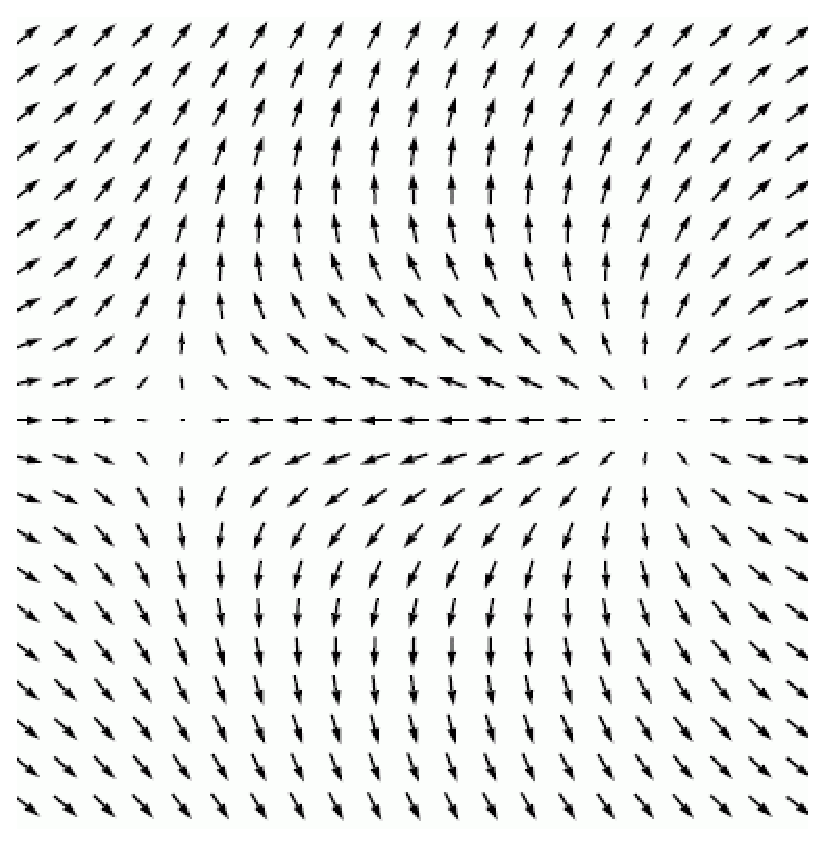
\includegraphics[scale=0.45]{vortices4.eps}
\end{figure}
Topological defect pairs pop in and out of the system and eventually unbind, 
leading to exponentially decaying correlations
}

%% 4 %%
\frame{
\frametitle{Crucial idea: order parameter space}
\begin{figure}
 \centering
 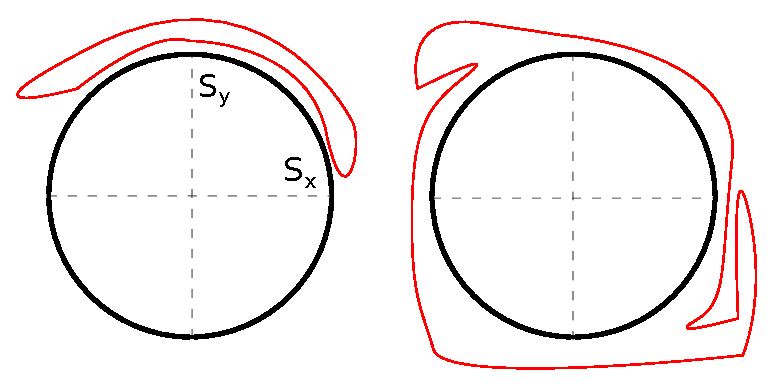
\includegraphics[scale=0.6]{topologicalspace.eps}
\end{figure}
Vortices are characterized by nontrivial winding around OP space.
}

%% 5 %%
\frame{
\frametitle{Conservation of topological charge}
\begin{itemize}
\item A lone vortex can be detected arbitrarily far away from the vortex core.
\item One single vortex has an energy that goes logarithmically with the size of the system: \emph{probability 0 in the thermodynamic limit.}
\item One +1 vortex is indistinguishable from two +1 vortices and a -1 vortex (from sufficiently far from the cores).
\item Therefore: \emph{there is a topological charge neutrality condition.} For every vortex spontaneously created, there is an anti vortex.
\end{itemize}
}

%% 6 %%
\frame{ 
\frametitle{HNY theory: Crystals}
\begin{itemize}
 \item Crystals are characterized by broken translational and rotational 
symmetry
\item Hexatic order parameter $\psi$ lives on a circle (1D torus) just like the XY model's order parameter.
\item Crystal displacement field $\bv u(\br_i)$ lives on a 2D torus: this is its order parameter space.
\end{itemize}
\begin{figure}
 \centering
 \includegraphics[scale=0.25]{OPspacecrystal.png}
\end{figure}
}

%% 7 %%
\frame{
\frametitle{Two types of topological defects in 2D crystals}
\begin{itemize}
 \item XY vortex $\goto$ winding number: disrupts spin-phase order
 \item Dislocation $\goto$ Burgers vector: disrupts translational order
 \item Disclination $\goto$ winding number: disrupts bond-orientational order
\end{itemize}
\begin{figure}
 \subfloat[Dislocations]{\includegraphics[scale=0.3]{pointdefects.png} } \quad
 \subfloat[Disclinations]{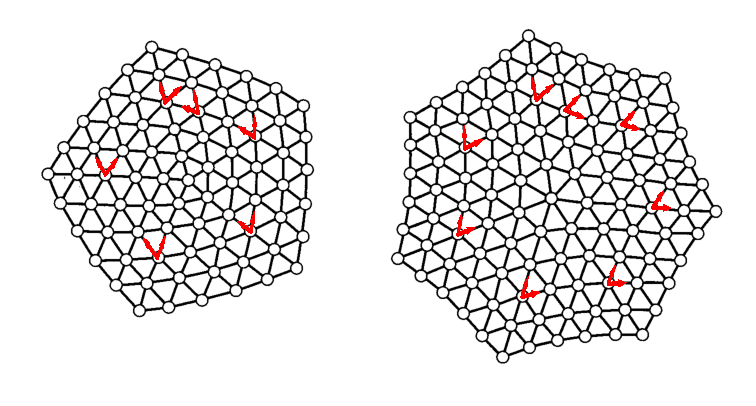
\includegraphics[scale=0.6]{disclinations.eps} }
\end{figure}

}

%% 8 %%
\frame{ 
\frametitle{Phase transitions in 2D \emph{rely} on topological defects}
\begin{itemize}
 \item What distinguishes a disordered system from one that hasn't ``melted'' 
in two dimensions?
 \begin{itemize}
 \item Stiffness (non-infinite susceptibility for XY, non-zero elastic 
constants for crystals)
 \item Stiffnesses are renormalized by the presence of defects
 \item Power-law correlations (as opposed to exponential correlations)
 \end{itemize}
 \item They won't show up in the Hamiltonian unless you:
 \begin{itemize}
 \item understand the symmetries of the original, unapproximated Hamiltonian
 \item account for the topology of the order parameter space
 \end{itemize}
\end{itemize}
}

%% 9 %%
\frame{
\frametitle{Interactions of defects}
\begin{itemize}
 \item KTHNY theory says defects show Coulombic attraction.
 \begin{itemize}
  \item In 2D, Coulomb energy is not $1/r$ but $\log r$ instead.
  \item Dislocations are vector charges, disclinations are scalar charges.
 \end{itemize}
 \item Costs energy to create the core of a defect/anti-defect pair, then costs more energy to separate them.
\end{itemize}

Now for some actual data...
}

%% FIGURESSSSS FAH DAAAAAYS %%

%% 10 %%
\frame{
\frametitle{$\phi=0.710$, $N=50^2$}
\begin{figure}
\centering
 \includegraphics[scale=1.4]{phi071_bounddislocations.pdf}
\end{figure}
$\phi = 0.710$, a few dislocation/anti-dislocation pairs. One dislocation 
triplet. Unbinding is extremely unfavorable.
}

%% 11 %%
\frame{ 
\frametitle{$\phi=0.700$, clustering, dislocation unbinding}
\begin{figure}
 \centering
 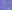
\includegraphics[scale=1.1]{phi070_stringofdefects.pdf}
\end{figure}
}

%% 12 %%
\frame{ 
\frametitle{$\phi=0.685$, hexatic domain walls}
\begin{figure}
 \centering
 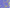
\includegraphics[scale=1.1]{phi0685_boundaries.pdf}
\end{figure}
}

%% 13 %%
\frame{ 
\frametitle{$\phi=0.685$, well in the hexatic phase}
\begin{figure}
 \centering
 \includegraphics[scale=1.2]{phi0685_hexaticphase.pdf}
\end{figure}
}

%% 14 %%
\frame{
\frametitle{$\phi=0.680$, disclination unbinding}
\begin{figure}
 \centering
 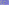
\includegraphics[scale=1.2]{phi068_antivortex.pdf}
\end{figure}
}

%% 15 %%
\frame{
\frametitle{$\phi=0.680$, disclination unbinding}
\begin{figure}
 \centering
 
\includegraphics[scale=1.2]{phi068_vortexpairs.pdf}
\end{figure}
}

%% 16 %%
\frame{
\frametitle{$\phi=0.680$, disclination unbinding}
\begin{figure}
 \centering
 
\includegraphics[scale=1.2]{phi068_netvortices.pdf}
\end{figure}
}

%% 17 %%
\frame{ 
\frametitle{$\phi=0.670$, $N=128^2$}
\begin{figure}
 \centering
 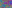
\includegraphics[scale=1.35]{phi067_N16000_color.pdf}
\end{figure}
}

%% 18 %%
\frame{
\frametitle{Phonon/libron modes: defects affect stiffness 
constants}
Light blue: phonon elastic stiffness. Red: libron elastic stiffness. Blue: 
libron mass. Green: libron-phonon coupling (0 by symmetry).
\begin{figure}
\captionsetup[subfigure]{labelformat=empty}
 \subfloat[$\phi$]{\includegraphics[scale=0.3]{couplings_zoom.png} }
 \subfloat[$\phi$]{\includegraphics[scale=0.3]{libcouplings_zoom.png} }
\end{figure}
}



\end{document}